\section{Zobrazení nižších LOD}
\label{sec-LODdisplay}
Zásadním problémem, který je nutné v rámci korektního zobrazování nižších LOD vyřešit, je správné zpracování průhlednosti. Průhlednost je podstatná z několika důvodů:
\begin{itemize}
\item skrývání řezů skoro rovnoběžných s pohledem
\item přechod mezi úrovněmi
\item lepší zobrazení samotného řezu
\end{itemize}
Korektní zpracování průhlednosti při přímé rasterizaci však není v rámci GPU automaticky ošetřeno. Proto je nutné věnovat zobrazování průhledné geometrie zvláštní pozornost. Nejběžnější metodou, která dokáže zobrazovat většinu možných případů prostorových uspořádání průhledných objektů správně, je tzv. \emph{malířův algoritmus}, který vykresluje objekty v pořadí od nejvzdálenějšího k nejbližšímu. Nevýhodou je, že je nutné řadit grafická primitiva (\emph{back-to-front ordering}). V poslední době s rostoucími možnostmi grafického hardware bylo představeno i několik tzv. \emph{order-independent} % citovat order-independent transparency
 technik. Uveďme zejména \cite{order-independent}, která je však zatím vázaná na technologii DirectX 11. Další možností je \emph{multisampling} s technikou \emph{alpha-to-coverage}. Využívá vícenásobného vzorkování pixelu obrazu a průhlenost zde řídí, kolik vzorků bude pokryto právě kresleným průhledným objektem. Ačkoliv má tato metoda relativně slibný teoretický základ (výsledek je tím lepší, čím více vzorků použijeme), v praxi často hardware umožňuje vzorkování nanejvýš 16 vzorků. Rozsah běžných průhledností [0\dots255] se tím sníží na 16 hodnot.

Ošetření problémů spojených s průhledností lze rozdělit do dvou skupin:
\begin{itemize}
\item průhlednost v rámci jedné instance
\item průhlednost v rámci instancí mezi sebou
\end{itemize}

\begin{figure}[!hbt]
\begin{center}
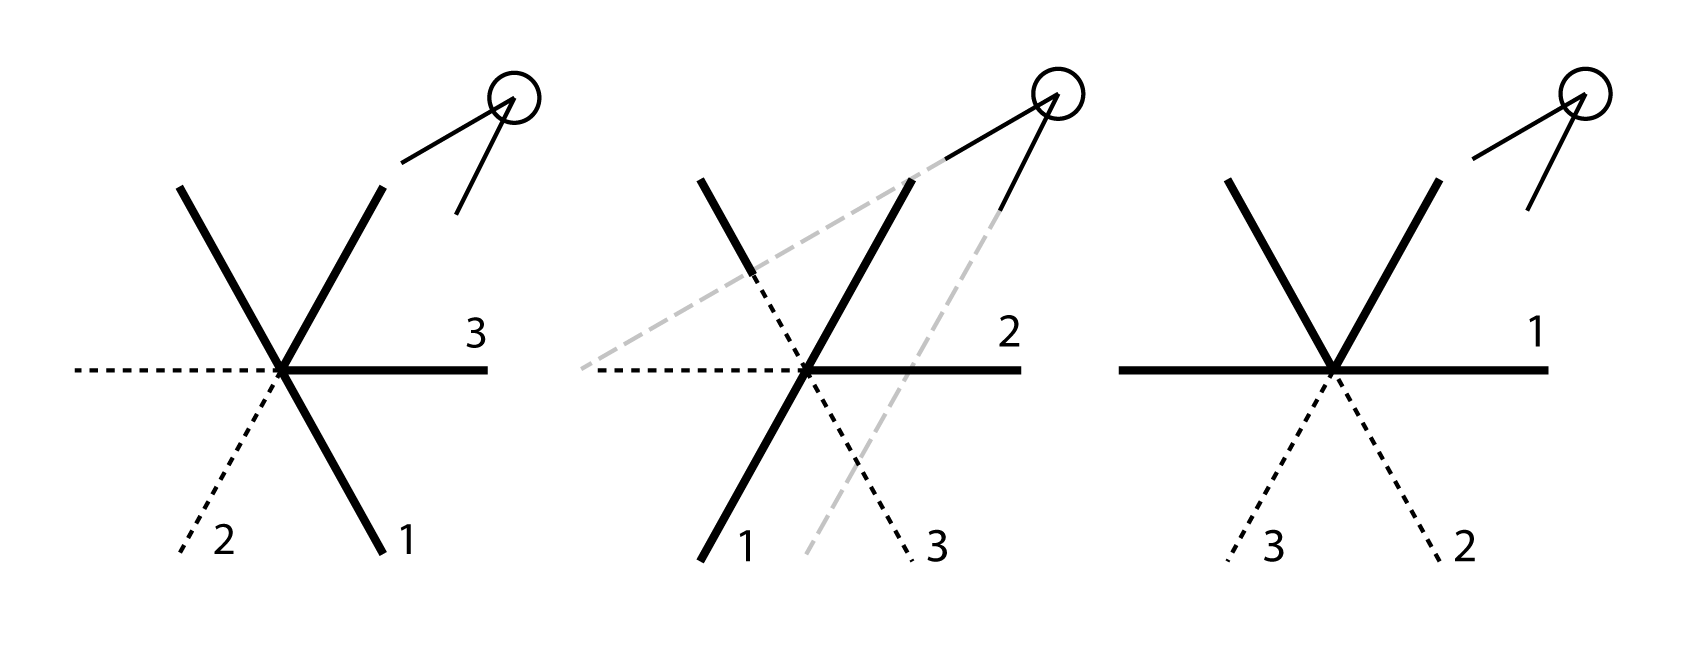
\includegraphics[width=0.6\textwidth]{./figures/LODtransparency.png}
\end{center}
\caption[Průhlednost trsu řezů]%
{Schematicky znázorněné problémy vykreslování průhledných, křížících se řezů. Tlustou plnou čarou jsou naznačeny správně vykreslené oblasti, tence čárkovaně oblasti, které nejsou vykresleny a mohou způsobit problémy.
\label{fig:lodSliceOrdering}
}
\end{figure}

Průhlednost mezi instancemi je ošetřena řazením v rámci zpracování instancí. Geometrická primitiva v rámci jedné instance je ovšem také třeba řadit. Jak je patrné z obrázku \ref{fig:lodSliceOrdering}, nelze pouhým řazením geometrických primitiv zajistit zcela korektní vykreslení. Ovšem důležité je si uvědomit skutečnost, že problémy způsobují zejména řezy skoro rovnoběžné s pohledem (dále jen \emph{rovnoběžný řez}), které jsou stejně skrývány (proto jsou vysoce průhledné). Zejména problematická je pak jejich část blíž k pozorovateli. Část dále od pozorovatele zakrývají řezy méně průhledné natočené víceméně kolmo ke směru pohledu. Stačí tedy zajistit, aby se takový rovnoběžný řez vykresloval až po ostatních.
\begin{figure}[!hbt]
\begin{center}
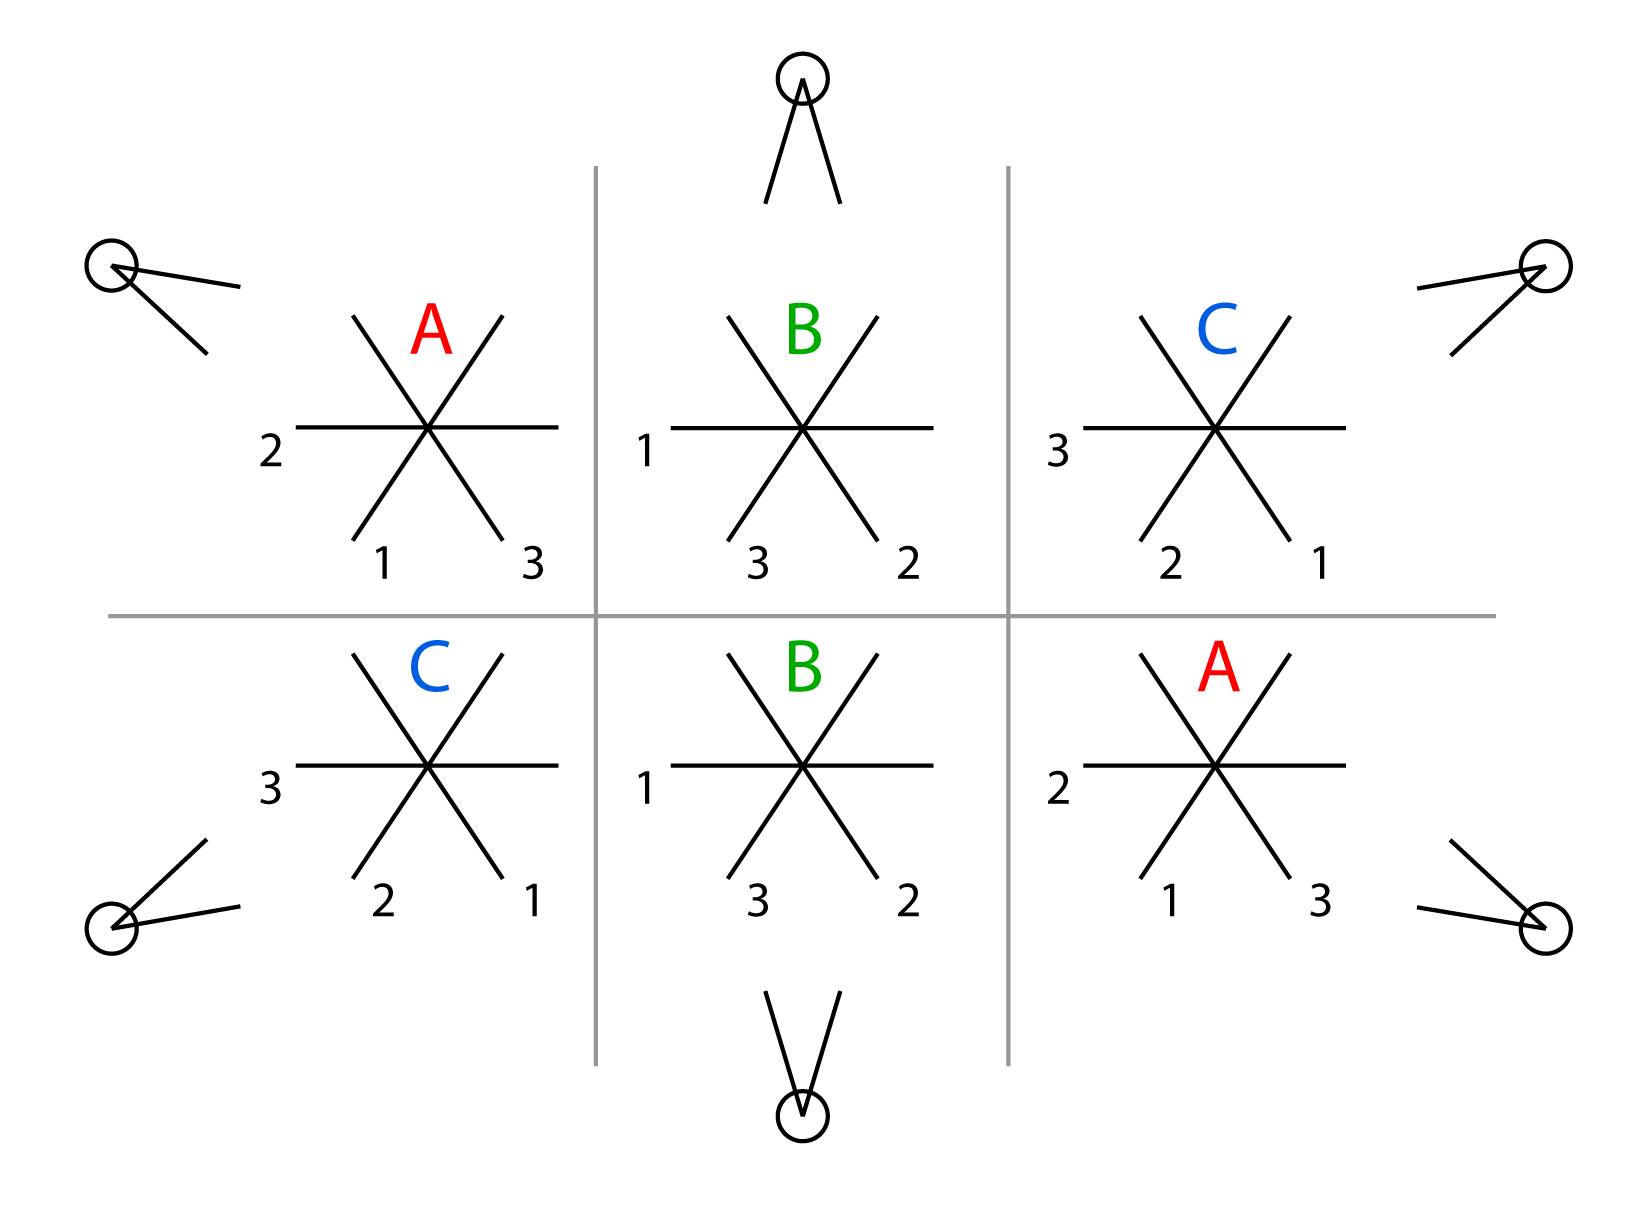
\includegraphics[width=0.6\textwidth]{./figures/LODtypes.png}
\end{center}
\caption[Variace pořadí vykreslování trsu řezů]%
{Různé případy pozice pozorovatele vůči trsu řezů. Všechny možnosti se redukují na 3 případy pořadí vykreslování řezů (A,B,C).
\label{fig:LODtypes}
}
\end{figure}
Jak je patrné z obr.~\ref{fig:LODtypes}, je třeba rozlišit, jaký případ nastává a podle toho určit pořadí vykreslení jednotlivých řezů. Fronty instancí se tedy rozpadají ještě podle tohoto kritéria (viz obr. \ref{fig:LODqueues}), neboť různé pořadí vykreslení jednotlivých řezů je zajištěno různým souborem indexů v EBO.
\begin{figure}[!hbt]
\begin{center}
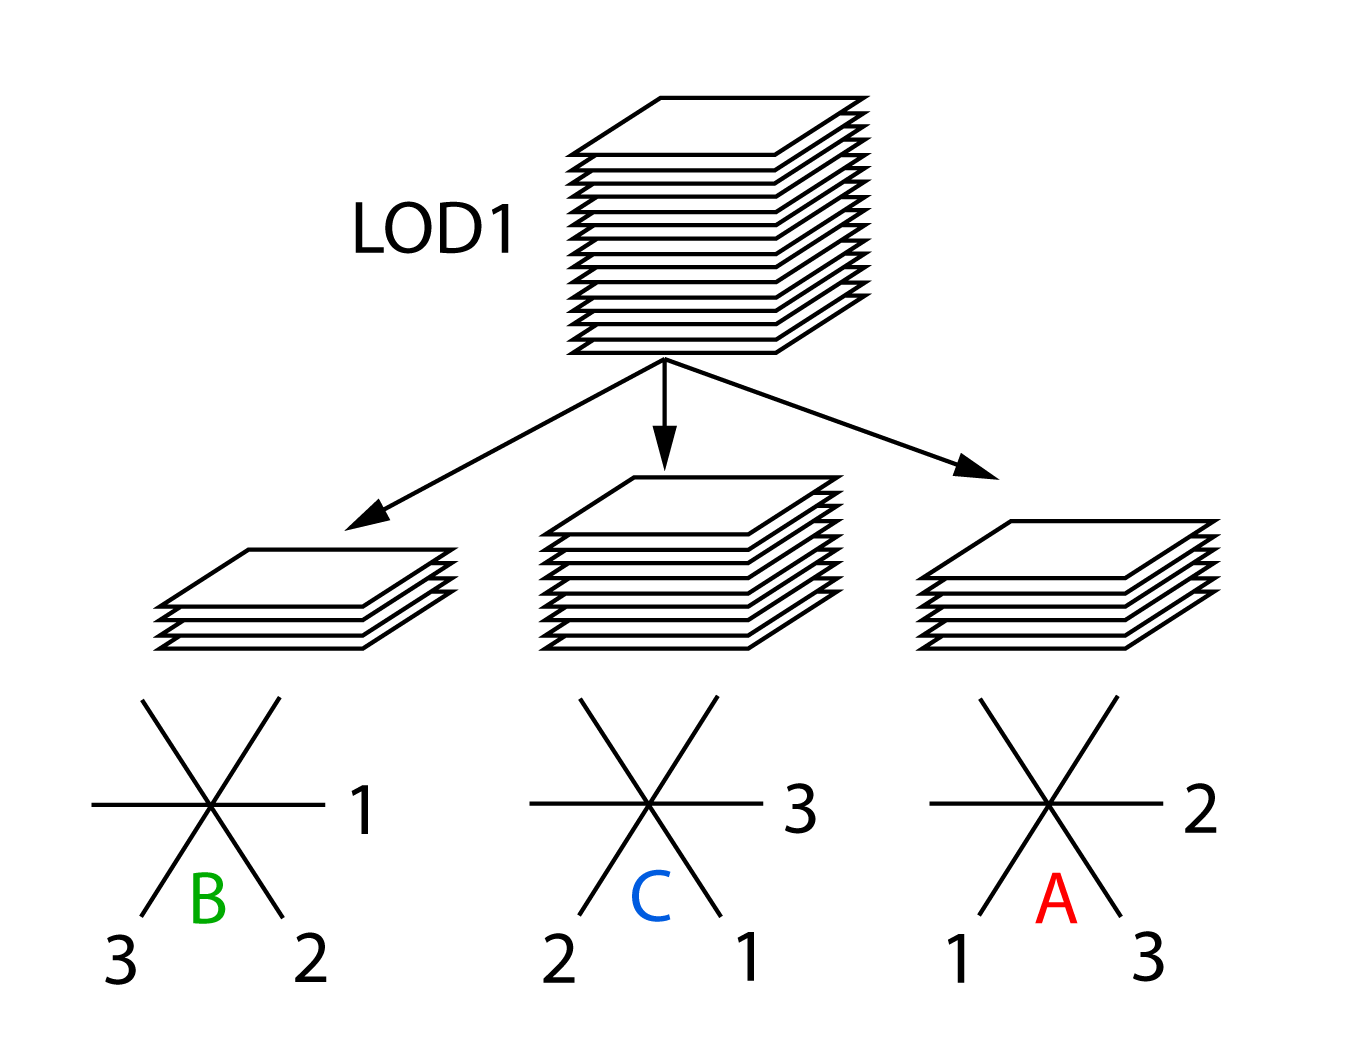
\includegraphics[width=0.4\textwidth]{./figures/renderQueuesB.png}
\end{center}
\caption[Pořadí vykreslování LOD1]%
{Rozpad fronty instancí LOD1 do několika menších front podle pořadí vykreslení (A,B,C).
\label{fig:LODqueues}
}
\end{figure}



\begin{itemize}
\item skrývání - řízení průhlednosti
\item pořadí vykreslování primitiv \& instancování (viz architektura LOD)
\item stíny
\end{itemize}